\documentclass[a4paper, twocolumn]{article}
\usepackage[pdftex, hidelinks]{hyperref}

\usepackage{bm}
\usepackage[T1]{fontenc}
\usepackage[utf8]{inputenc}
\usepackage{algorithmic}
\usepackage{algorithm}
\usepackage{amsfonts}
\usepackage{amssymb}
\usepackage{courier}
\usepackage{booktabs}
\usepackage{graphicx}
\usepackage{listings}
\usepackage{mathtools}
\usepackage{amssymb}
\lstset{basicstyle=\footnotesize\ttfamily,
        breakatwhitespace = false,
        breaklines = true,
        keepspaces = true,
        language = R,
        showspaces = false,
        showstringspaces = false,
        belowcaptionskip = \bigskipamount,
        framerule = 0.80pt,
        frame = tb,
        belowskip = \bigskipamount,
        escapeinside={<@}{@>}}

\title{TDDE01 -- Machine Learning \\
       Group 9 Laboration Report 4}
\author{{Martin Estgren \texttt{<mares480>}} \\
        {Erik S. V. Jansson \texttt{<erija578>}} \\
        {Sebastian Maghsoudi \texttt{<sebma654>}} \\~\\
        {Linköping University (LiU), Sweden}}

\begin{document}
    \pagenumbering{arabic}
    \maketitle % Generate.

    \section*{Assignment 1}
    This assignment involves examining a given data set called \emph{State}, which contains the observations about the \emph{population} \& \emph{economy} in different \emph{states}. We are primarily interested in the relationship between the \emph{metropolitan habitation rate (MET)} and the \emph{public expenditure per capita (EX)} for a given state.

    \subsection{Raw data analysis}

    We first analyze the data by plotting the \emph{EX} target as a function of \emph{MET}. This plot can be observed in Figure~\ref{fig:state}.

        \begin{figure}[h!]
          \centering
          \caption{Plot of MET vs EX}
          \label{fig:state}
          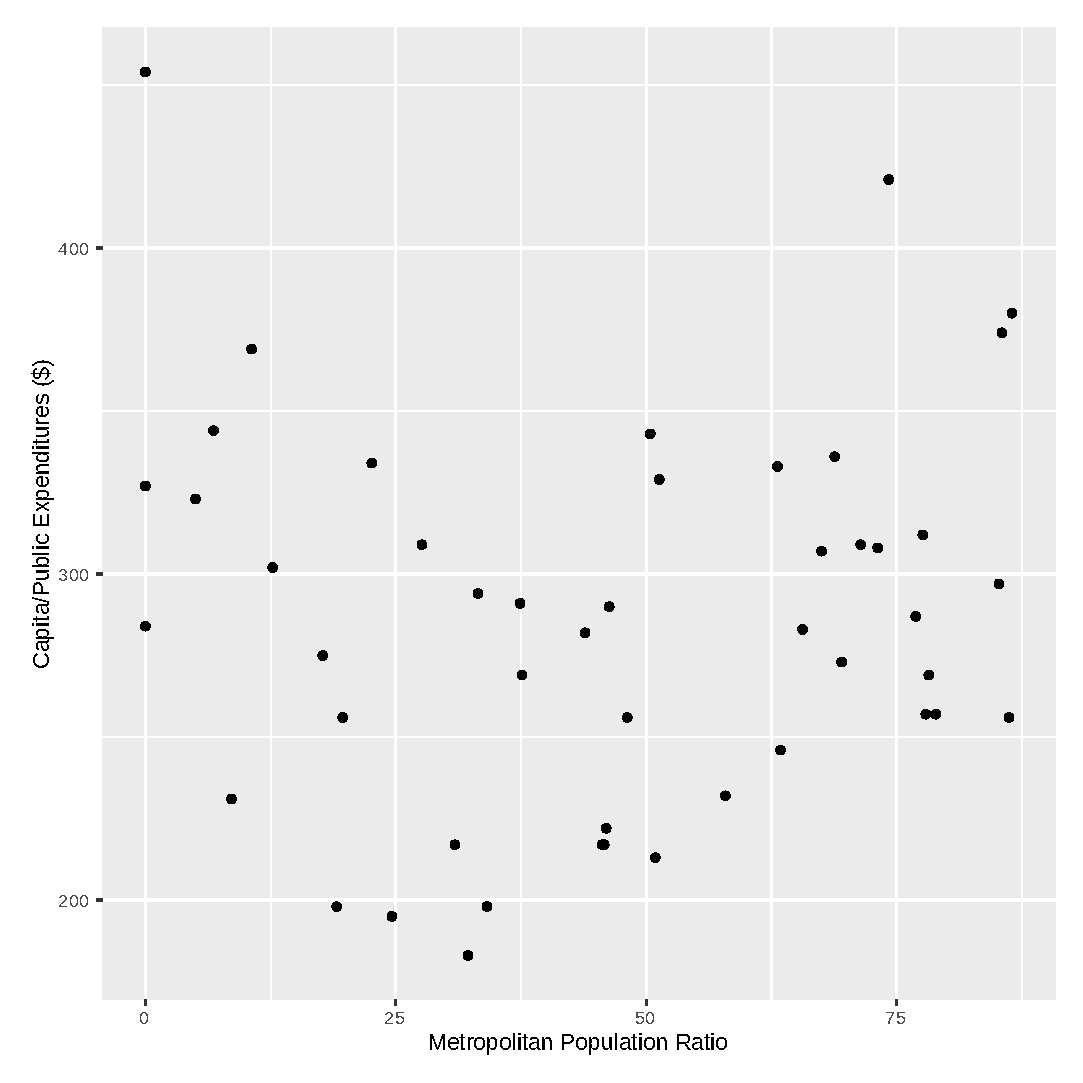
\includegraphics[width=0.5\textwidth]{share/state.eps}
        \end{figure}

    The figure indicates that a linear model isn't suitable for predicting the target in this data set, no visible pattern can be observed.

    \subsection{Regression tree}

    We have examined how a \emph{regression tree model} fits the data set using \emph{cross-validation} for finding the optimal number of \emph{leaves}. The plotted \emph{tree} from the fitted model can be seen in Figure~\ref{fig:tree.eps}. According to the cross-validation, the optimal number of leaves is 3, which we use to prune the full tree model and get the best optimal model. The predicted results can be seen in Figure~\ref{fig:predicted}.

        \begin{figure}[h!]
          \centering
          \caption{Plot of MET vs Predicted EX}
          \label{fig:state}
          \includegraphics[width=0.5\textwidth]{share/predicted.eps}
        \end{figure}
        As can be seen, the predictions have less labels compared to the original data. 

        The frequency of the models residuals are displayed in the histogram \ref{fig:residuals}.

        \begin{figure}[h!]
          \centering
          \caption{Histogram of residuals}
          \label{fig:state}
          \includegraphics[width=0.5\textwidth]{share/residuals.eps}
        \end{figure}
        \texbf{Fluff!}


    \subsection{non-parametric bootstrap}
    
    We examine the same data set with a \emph{regression tree model} with \emph{non-parametric bootstrap}. The model will follow the same structure as above but use \emph{bootstrapping} instead of \emph{cross-validation}.
   
    The \emph{non-parametric bootstrap} re-samples the given data set $1000$ times and estimate the model based on the \emph{regression tree model}. We examine the confidence band of the predicted model with a confidence level of 0.95 (fig \ref{fig:confidence_bound}).
        
        \begin{figure}[h!]
          \centering
          \caption{Confidence bound of the regression tree model}
          \label{fig:confidence_bound}
          \includegraphics[width=0.5\textwidth]{share/confidence_bound.eps}
        \end{figure}
            

    \subsection{parametric bootstrap}
    \begin{itemize}
        \item Show the parametric function
        \item Show the bootstrap function
        \item Show the confidence and prediction bounds
        \item Questions
    \end{itemize}
    \section*{Assignment 2}
    Fluff
    \subsection{Principle component analysis}
    \begin{itemize}
        \item Show the data 
        \item Show the PCA function (which components were chosen?)
        \item Show the trace plot and loadings plot
        \item Questions
    \end{itemize}
    \subsection{Independent component analysis}
    \begin{itemize}
        \item Show the ICA function (which components were chosen?)
        \item Show the trace and loadings plot
        \item Questions
    \end{itemize}
    \subsection{Cross validation for PCA}
    \begin{itemize}
        \item Show the cross validation function
        \item Show the result?
        \item Questions
    \end{itemize}
    \nocite{*} % No warnings.
    \bibliographystyle{alpha}
    \bibliography{report}
    \onecolumn \appendix
    \section*{Appendix}


\end{document}
